\section{Computational Bounds and Visualizations}\label{app:computational}

Exhaustive enumeration of connected subgraphs becomes intractable beyond $R=7$.
Figure~\ref{fig:complexity} illustrates the efficiency of our $O(R^3 \log R)$
characterization engine compared to brute-force search (which grows as
$\Omega(R^{R-2})$), enabling exact boundary computation for arbitrary $R$.

\begin{figure}[H]
	\centering
	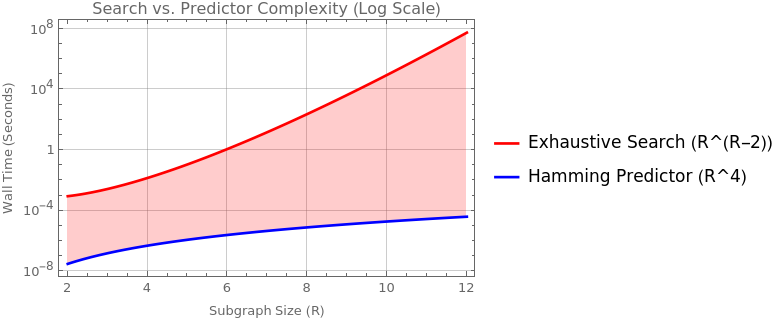
\includegraphics[width=0.8\textwidth]{../docs/complexity-curves.pdf}
	\caption{The combinatorial growth of state-space search versus our
	$O(R^3 \log R)$ engine mapping limits up to and beyond $R=128$.}
	\label{fig:complexity}
\end{figure}

Figures~\ref{fig:r9} and~\ref{fig:r10} show the induced subgraph structure of
$\mathrm{HB}_R$ for $R = 9$ and $R = 10$. Because the Hamming Ball is defined by
binary strings, this structure is independent of the host graph $A(n,k)$
(provided $n-k \ge 4$ and $k \ge 4$). Both extend the perfect $Q_3$ cube ($R=8$)
by adding vertices that share the maximum number of roots with the existing
ball.

\begin{figure}[H]
	\centering
	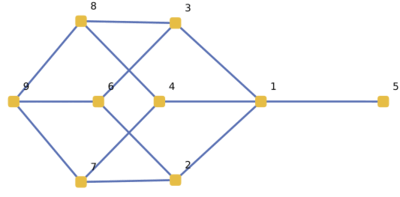
\includegraphics[width=0.5\textwidth]{../assets/out/R9_graph.png}
	\caption{Induced subgraph of $\mathrm{HB}_9$: the $Q_3$ cube plus one
	vertex, yielding $D = 13$. Valid for any $A(n,k)$ with $n-k \ge 4$,
	$k \ge 4$.}
	\label{fig:r9}
\end{figure}

\begin{figure}[H]
	\centering
	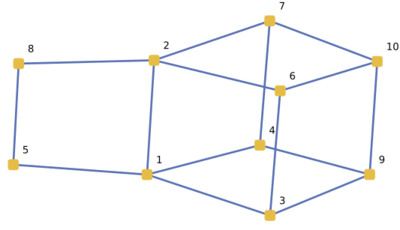
\includegraphics[width=0.5\textwidth]{../assets/out/R10_graph.png}
	\caption{Induced subgraph of $\mathrm{HB}_{10}$: the $Q_3$ cube plus two
	vertices, yielding $D = 15$. Valid for any $A(n,k)$ with $n-k \ge 4$,
	$k \ge 4$.}
	\label{fig:r10}
\end{figure}

\begin{table}[H]
	\centering
	\caption{Exact minimum-cut bounds ($R=2$ to $R=130$)}
	\small
	\begin{tabular}{ccc|ccc|ccc}
		\toprule
		$R$ & $\Eseq(R)$ & $\Cconst(R)$ & $R$ & $\Eseq(R)$ & $\Cconst(R)$ & $R$ & $\Eseq(R)$ & $\Cconst(R)$ \\
		\midrule
		2   & 1          & 1            & 45  & 115        & 136          & 88  & 268        & 308          \\
		3   & 2          & 3            & 46  & 119        & 139          & 89  & 271        & 313          \\
		4   & 4          & 4            & 47  & 123        & 142          & 90  & 275        & 317          \\
		5   & 5          & 7            & 48  & 128        & 144          & 91  & 279        & 321          \\
		6   & 7          & 9            & 49  & 130        & 149          & 92  & 284        & 324          \\
		7   & 9          & 11           & 50  & 133        & 153          & 93  & 288        & 328          \\
		8   & 12         & 12           & 51  & 136        & 157          & 94  & 293        & 331          \\
		9   & 13         & 16           & 52  & 140        & 160          & 95  & 298        & 334          \\
		10  & 15         & 19           & 53  & 143        & 164          & 96  & 304        & 336          \\
		11  & 17         & 22           & 54  & 147        & 167          & 97  & 306        & 342          \\
		12  & 20         & 24           & 55  & 151        & 170          & 98  & 309        & 347          \\
		13  & 22         & 27           & 56  & 156        & 172          & 99  & 312        & 352          \\
		14  & 25         & 29           & 57  & 159        & 176          & 100 & 316        & 356          \\
		15  & 28         & 31           & 58  & 163        & 179          & 101 & 319        & 361          \\
		16  & 32         & 32           & 59  & 167        & 182          & 102 & 323        & 365          \\
		17  & 33         & 37           & 60  & 172        & 184          & 103 & 327        & 369          \\
		18  & 35         & 41           & 61  & 176        & 187          & 104 & 332        & 372          \\
		19  & 37         & 45           & 62  & 181        & 189          & 105 & 335        & 377          \\
		20  & 40         & 48           & 63  & 186        & 191          & 106 & 339        & 381          \\
		21  & 42         & 52           & 64  & 192        & 192          & 107 & 343        & 385          \\
		22  & 45         & 55           & 65  & 193        & 199          & 108 & 348        & 388          \\
		23  & 48         & 58           & 66  & 195        & 205          & 109 & 352        & 392          \\
		24  & 52         & 60           & 67  & 197        & 211          & 110 & 357        & 395          \\
		25  & 54         & 64           & 68  & 200        & 216          & 111 & 362        & 398          \\
		26  & 57         & 67           & 69  & 202        & 222          & 112 & 368        & 400          \\
		27  & 60         & 70           & 70  & 205        & 227          & 113 & 371        & 405          \\
		28  & 64         & 72           & 71  & 208        & 232          & 114 & 375        & 409          \\
		29  & 67         & 75           & 72  & 212        & 236          & 115 & 379        & 413          \\
		30  & 71         & 77           & 73  & 214        & 242          & 116 & 384        & 416          \\
		31  & 75         & 79           & 74  & 217        & 247          & 117 & 388        & 420          \\
		32  & 80         & 80           & 75  & 220        & 252          & 118 & 393        & 423          \\
		33  & 81         & 86           & 76  & 224        & 256          & 119 & 398        & 426          \\
		34  & 83         & 91           & 77  & 227        & 261          & 120 & 404        & 428          \\
		35  & 85         & 96           & 78  & 231        & 265          & 121 & 408        & 432          \\
		36  & 88         & 100          & 79  & 235        & 269          & 122 & 413        & 435          \\
		37  & 90         & 105          & 80  & 240        & 272          & 123 & 418        & 438          \\
		38  & 93         & 109          & 81  & 242        & 278          & 124 & 424        & 440          \\
		39  & 96         & 113          & 82  & 245        & 283          & 125 & 429        & 443          \\
		40  & 100        & 116          & 83  & 248        & 288          & 126 & 435        & 445          \\
		41  & 102        & 121          & 84  & 252        & 292          & 127 & 441        & 447          \\
		42  & 105        & 125          & 85  & 255        & 297          & 128 & 448        & 448          \\
		43  & 108        & 129          & 86  & 259        & 301          & 129 & 449        & 456          \\
		44  & 112        & 132          & 87  & 263        & 305          & 130 & 451        & 463          \\
		\bottomrule
	\end{tabular}
\end{table}

\subsection{CP-SAT diagnostic searches}

In addition to exhaustive enumeration, the repository contains bounded
CP-SAT models intended as adversarial diagnostics, not as substitutes for a
universal proof.  The single-fiber model optimizes the exact collision and
defect quantities and can fix a defect shortfall.  It also reports the
proposition-equivalent residual
\[X-\bigl(\Cconst(R)-\Eseq(R)\bigr)-(m+1)\bigl(\Eseq(R)-D\bigr).
\]
The tripartite model optimizes the third-order boundary interface used in
Lemma~\ref{lem:interface-subadditivity}.  A coordinate-local model maximizes
the empty-slice residual described in Appendix~\ref{app:alt-strategies}.

For all such searches, an \texttt{OPTIMAL} status certifies the stated optimum
only for that finite $(n,k,R)$ instance; a \texttt{FEASIBLE} status is merely
an incumbent under the selected time limit.  The certified frontiers and their
witnesses are maintained in the accompanying research log.  They provide
counterexample hunting and structural examples, but do not verify
Proposition~\ref{prop:restricted_lower_bound} for arbitrary parameters.

\subsection{Exact Boolean model and certified floor}

For $A(10,5)$ the vertex set $V$ has $|V| = 30{,}240$ injective $5$-tuples.  The
model \texttt{a10\_5\_hunt} introduces per-vertex indicators: $x_v \in \{0,1\}$
with $x_v = 1$ iff $v \in S$, and $y_v \in \{0,1\}$ recording membership of $v$
in the external boundary set (exact under minimization).  The constraints
encode the set-theoretic definition of $\extbd$:
\begin{align}
	\sum_{v \in V} x_v &= 26, \label{eq:volume} \\
	x_v + y_v &\le 1 && \text{for all } v \in V, \label{eq:excl} \\
	y_v &\ge x_u - x_v && \text{for all } \{u,v\} \in E. \label{eq:bound-indicator}
\end{align}
For a fixed $x$, minimizing $\sum_v y_v$ drives $y_v$ to $0$ on selected
vertices and to $1$ exactly on external neighbors, so \eqref{eq:bound-indicator}
enforces $y_v = 1$ iff $v \in \extbd(S)$.  The model searches for subsets with
$\sum_v y_v \le \HuntTarget{}$ --- one below the $\SliceBoundary{}$-sized slice
witness --- under an imposed cutoff, and proves infeasibility iteratively.

\textbf{Global floor via a symmetry pin.}  A single vertex is pinned into $S$.
Since $A(10,5)$ is vertex-transitive, every $26$-subset is automorphic to one
containing the pinned vertex, and automorphisms preserve boundary size: a
certified floor on the pinned search is a certified floor over all subsets.
Core-guided conflict analysis has so far excluded every boundary size below
$\CertFloor{}$, and no feasible witness at or below $\HuntTarget{}$ has been
found (best = inf); the run archives more than $1.2$ million learned clauses,
each a localized geometric dead-end of $A(10,5)$.  The certified containment is
therefore
\[
	\CertFloor{} \le \min_{\substack{S \subseteq V\\ |S| = 26}} |\extbd(S)|
	\le \SliceBoundary{},
\]
with $\HuntTarget{}$ a search target rather than an upper bound.  This floor is
an evolving lower-bound record --- each successive core raises it --- and is
tracked in the accompanying research log.

\begin{remark}[Coordinate-edge counting]\label{rem:coord-edges}
Let $\CoordEdges(S)$ denote the total number of coordinate-aligned edges from
members of $S$ to the external boundary, counted per source coordinate:
$\CoordEdges(S) = \sum_{p=1}^{k} |\partial_p(S)|$, where $\partial_p(S)$ is the
set of external neighbors that differ from $S$ in position $p$.  Two exact
identities determine it from the defect-framework data alone:
\begin{equation}\label{eq:coord-edges}
	\CoordEdges(S) = |\extbd(S)| + X(S) = U(S)\,(m+1) - |S|\,k,
\end{equation}
where $U(S) = \sum_p |U_p(S)|$ is the total unique-root count
(eq.~\eqref{eq:unique-roots}), $m = n-k$, and
$X(S) = \CoordEdges(S) - |\extbd(S)|$ is the cross-collision surplus of
Section~\ref{sec:defect}: the excess of per-coordinate boundary incidences over
distinct boundary vertices.  The second equality counts, per occupied root
$r \in U(S)$, the $(m+1)$ vertices on its line minus those already selected
into $S$; every such external vertex is adjacent to all members on that line.
For the $26$-subsets of the bracket above, this ties the boundary size to a
single geometric count --- equivalently to the occupied-root count, since
$D(S) = k|S| - U(S)$.
\end{remark}
